\chapter{Methods}
\label{methods}

Predicting morphology and charge transport properties in OPVs is accomplished through the combination 
of techniques, each modeling specific physical phenomena.
In this section we outline the models and theory employed throughout the pipeline to describe 
the atomic structure of organic molecules, how they arrange, and how charges move through them. 
For each of these approaches, we then describe the open-source software tools that we create, modify, and use 
to implement these methods. 

In \autoref{md}, we introduce molecular simulation techniques used to predict self-assembly of OPVs.
In \autoref{marcusmodel}, we describe Marcus model of charge hopping between chromophores,
the techniques we use to identify individual chromophores in simulated volumes, 
and how we use quantum chemical calculations to estimate the Marcus hopping rate between
neighboring chromophores.
In \autoref{KMC}, we describe the basics of stochastically modeling kinetic processes and 
our specific kinetic Monte Carlo approach to modeling charge transport.
Finally, in \autoref{software-methods}, we enumerate the software used in this thesis and outline the means by
which it is developed. Particular focus is given to two packages that are principly developed by members of the CMELab:
\texttt{Planckton} and \texttt{MorphCT}.  
 

\section{Molecular Dynamics}

\label{md}

\begin{figure}
\centering
\begin{subfigure}{.5\textwidth}
    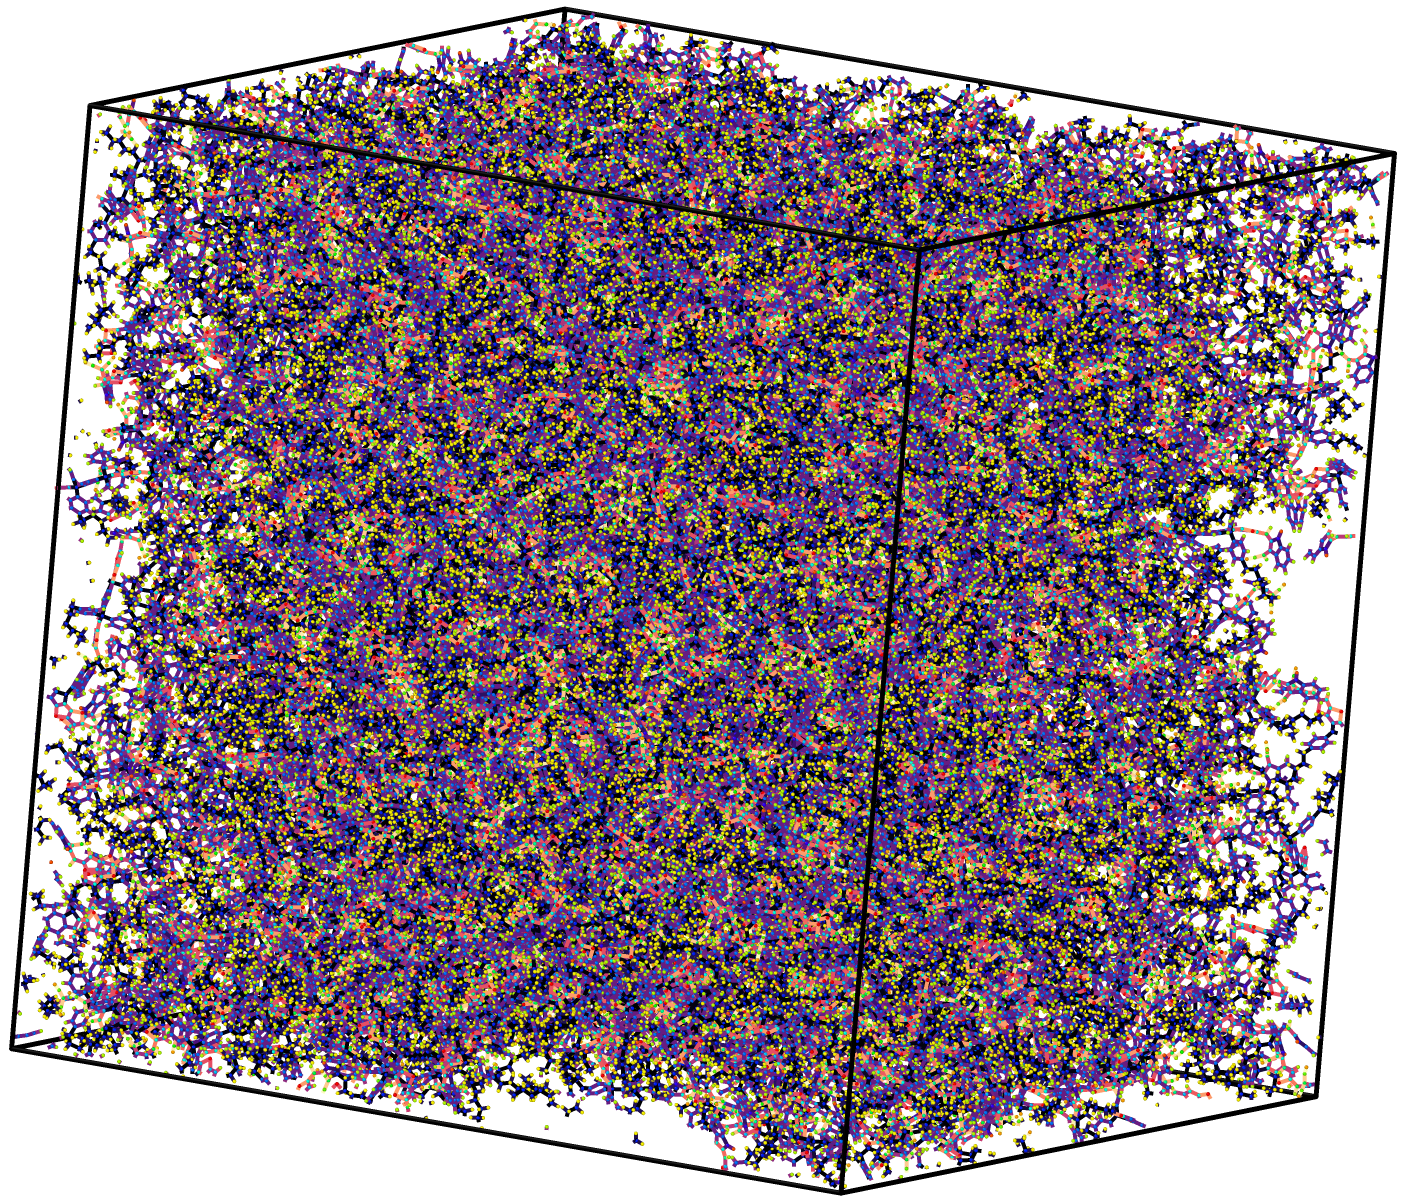
\includegraphics[width=\textwidth]{figures/consistent-color-itic.png}
\end{subfigure}%
\begin{subfigure}{.5\textwidth}
    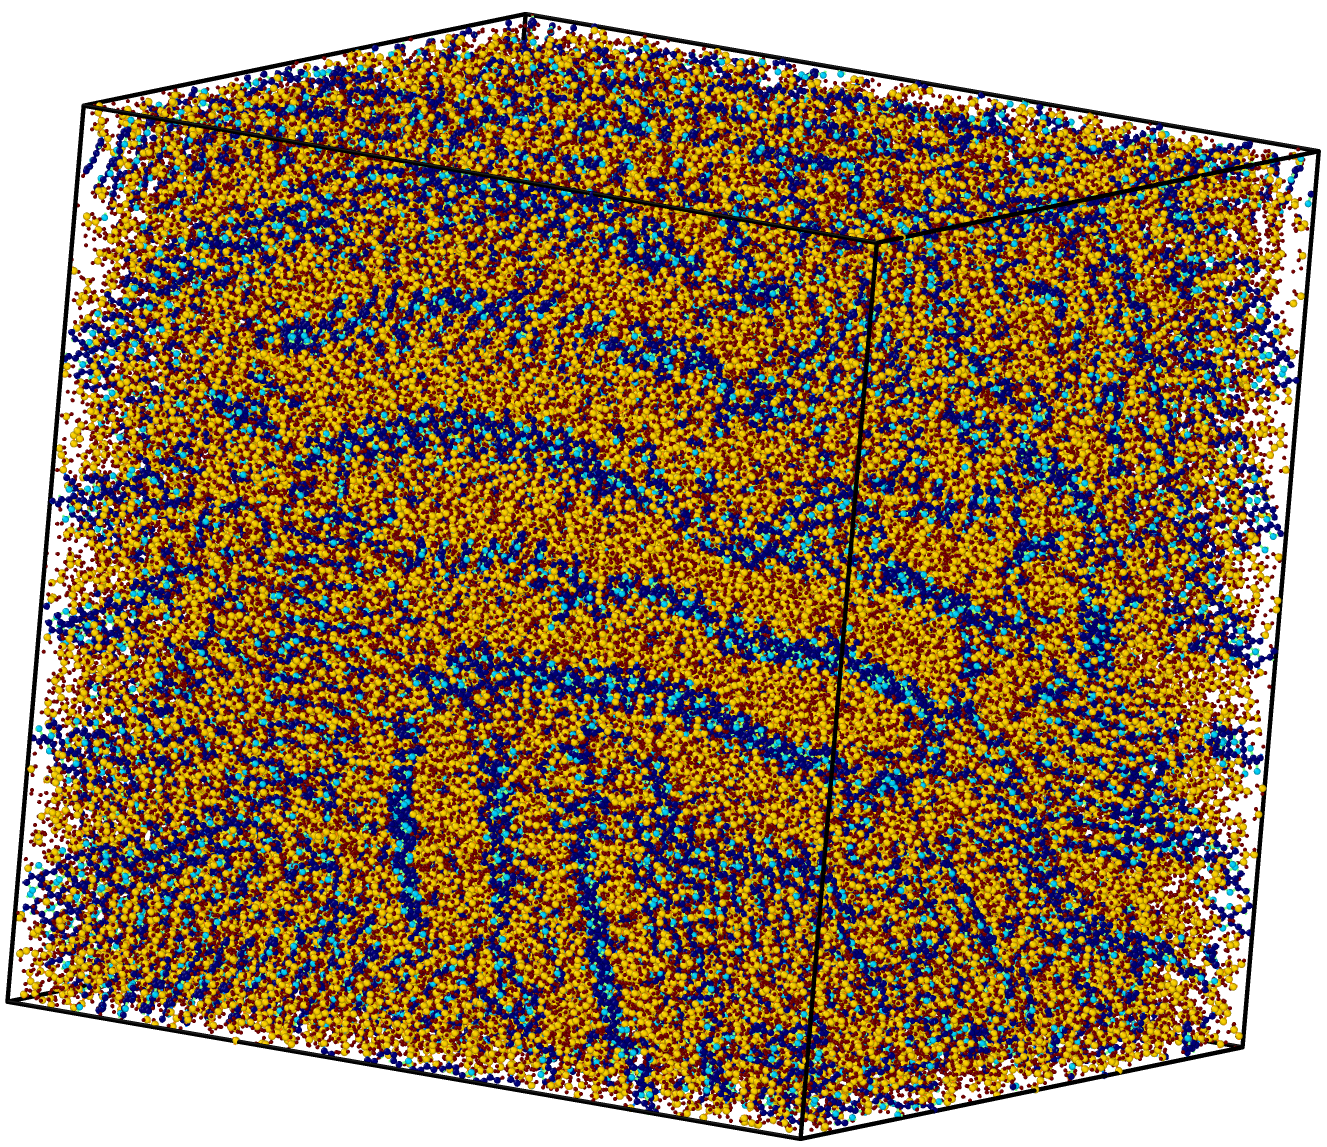
\includegraphics[width=\textwidth]{figures/consistent-color-p3ht.png}
\end{subfigure}
\\
\begin{subfigure}{.5\textwidth}
\centering
    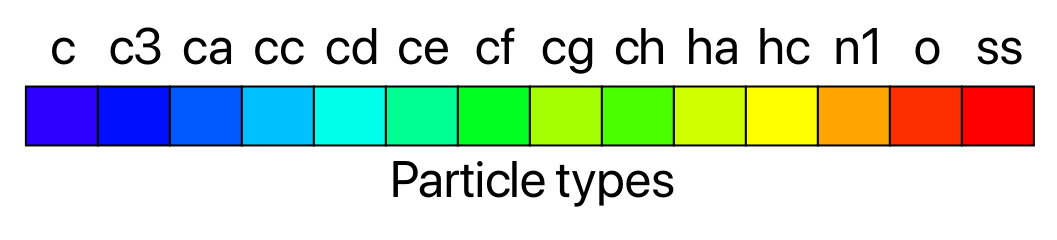
\includegraphics[width=.7\textwidth]{figures/itic-legend.png}
\end{subfigure}%
\begin{subfigure}{.5\textwidth}
\centering
    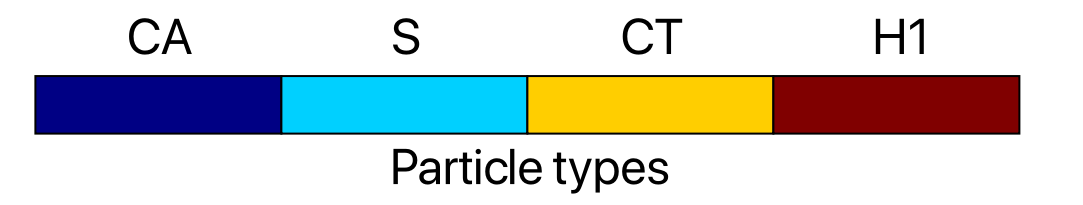
\includegraphics[width=.7\textwidth]{figures/color-legend-p3ht.png}
\end{subfigure}
    \caption[short]{Left: 1000 molecule atomistic morhology of ITIC. Right: 1000 oligomer atomistic simulation
    of P3HT
    }
\label{ITIC/P3HT}
\end{figure}

Modelling charge transport in OPVs demands a methodology that is accurate across orders of magnitude of
resolution. Electronic wave functions operate at the atomic scale while the morphological features (grain
boundaries, crystallinity etcetera) that govern charge transport occur across many nanometers. MD simulations
are suited to this task because they enable the combination of coarse-grained models with atomistic
representations to predict experimentally relevant length scales \cite{Miller2018}.

Molecular dynamics is a method of computer simulation for predicting the equilibrium geometries of molecular
systems. MD simulations proceed iteratively by solving Newtons laws of motion
in accordance with a predefined interatomic interaction potentials which define the forces between particles
in the system.  
The non-bonded ineraction potentials are modeled with a classic Leonard-Jones(LJ)
potential \cite{Jones1924a}. Potentials are also defined in accordance with the bonds that each particle is
participating in and can include parameteres for equillibrium bond distances and equillibrium angles between
$3$ bonded atoms and between $4$ bonded atoms (dihedral angles).
At each iteration, a numerical integation over these potentials provide an update to the velocities and positions
of particles in the system. 
\ej{Picture or cartoon of atoms, forces, and one update?}

Using the canonical ensemble (NVT) for example, conserving the number of
particles, the volume, and the temperature allows for the exploration of the potential energy surface
of the system and sample the microstates from equillibrated region the simulation for statistical analysis.  
Simulation ensembles are regulated via the Nos\'{e}-Hoover thermostat \cite{Hoover1985} to maintain 
temperature using the MTK equations \cite{Martyna1994d}\cite{Cao1996}.
The system can be considered equilibrated when the potential energy no longer decreases with time. 
From the the sum of all LJ potentials as the systems potential energy. Determining the equilibrated region of the
simulation can be fleshed out from the progression of the systems potential energy. By binning the microstates
into distinct regions, working backwards in time, a bin is added to the equillibrated region if its standard
deviation is less than twice that of the previous bin \cite{Henry2017a}.

MD simulations can predict the self-assembly of OPV materials. To connect the chemistry to the
conductivity of the material we use Marcus theory coupled with KMC.

\section{Marcus Model}
\label{marcusmodel}

The movement of a free charge through a morphology can be modeled as a series of 
Marcus nonadiabatic electron transfer
reactions, or `hops' between relatively weakly interacting chromophores in the system. 
Each hop then is modeled as a thermally activated process, the rate of which can be solved for analytically
from the interesction of two parabolic potential energy surfaces. 
Each parabola in \autoref{marcus-plot} represents the potential energy well of a charge that is localized on
one of two chromophores in a dimer complex. 
With electron transfer much much faster than the movement of nuclear coordinantes (Franck-Condon principle),
the intersection of the parabolas corresponds to the unique nuclear geometry, and distinct vibrational mode, at
which charge transfer is assumed to take place. 

\begin{figure}
  \center
  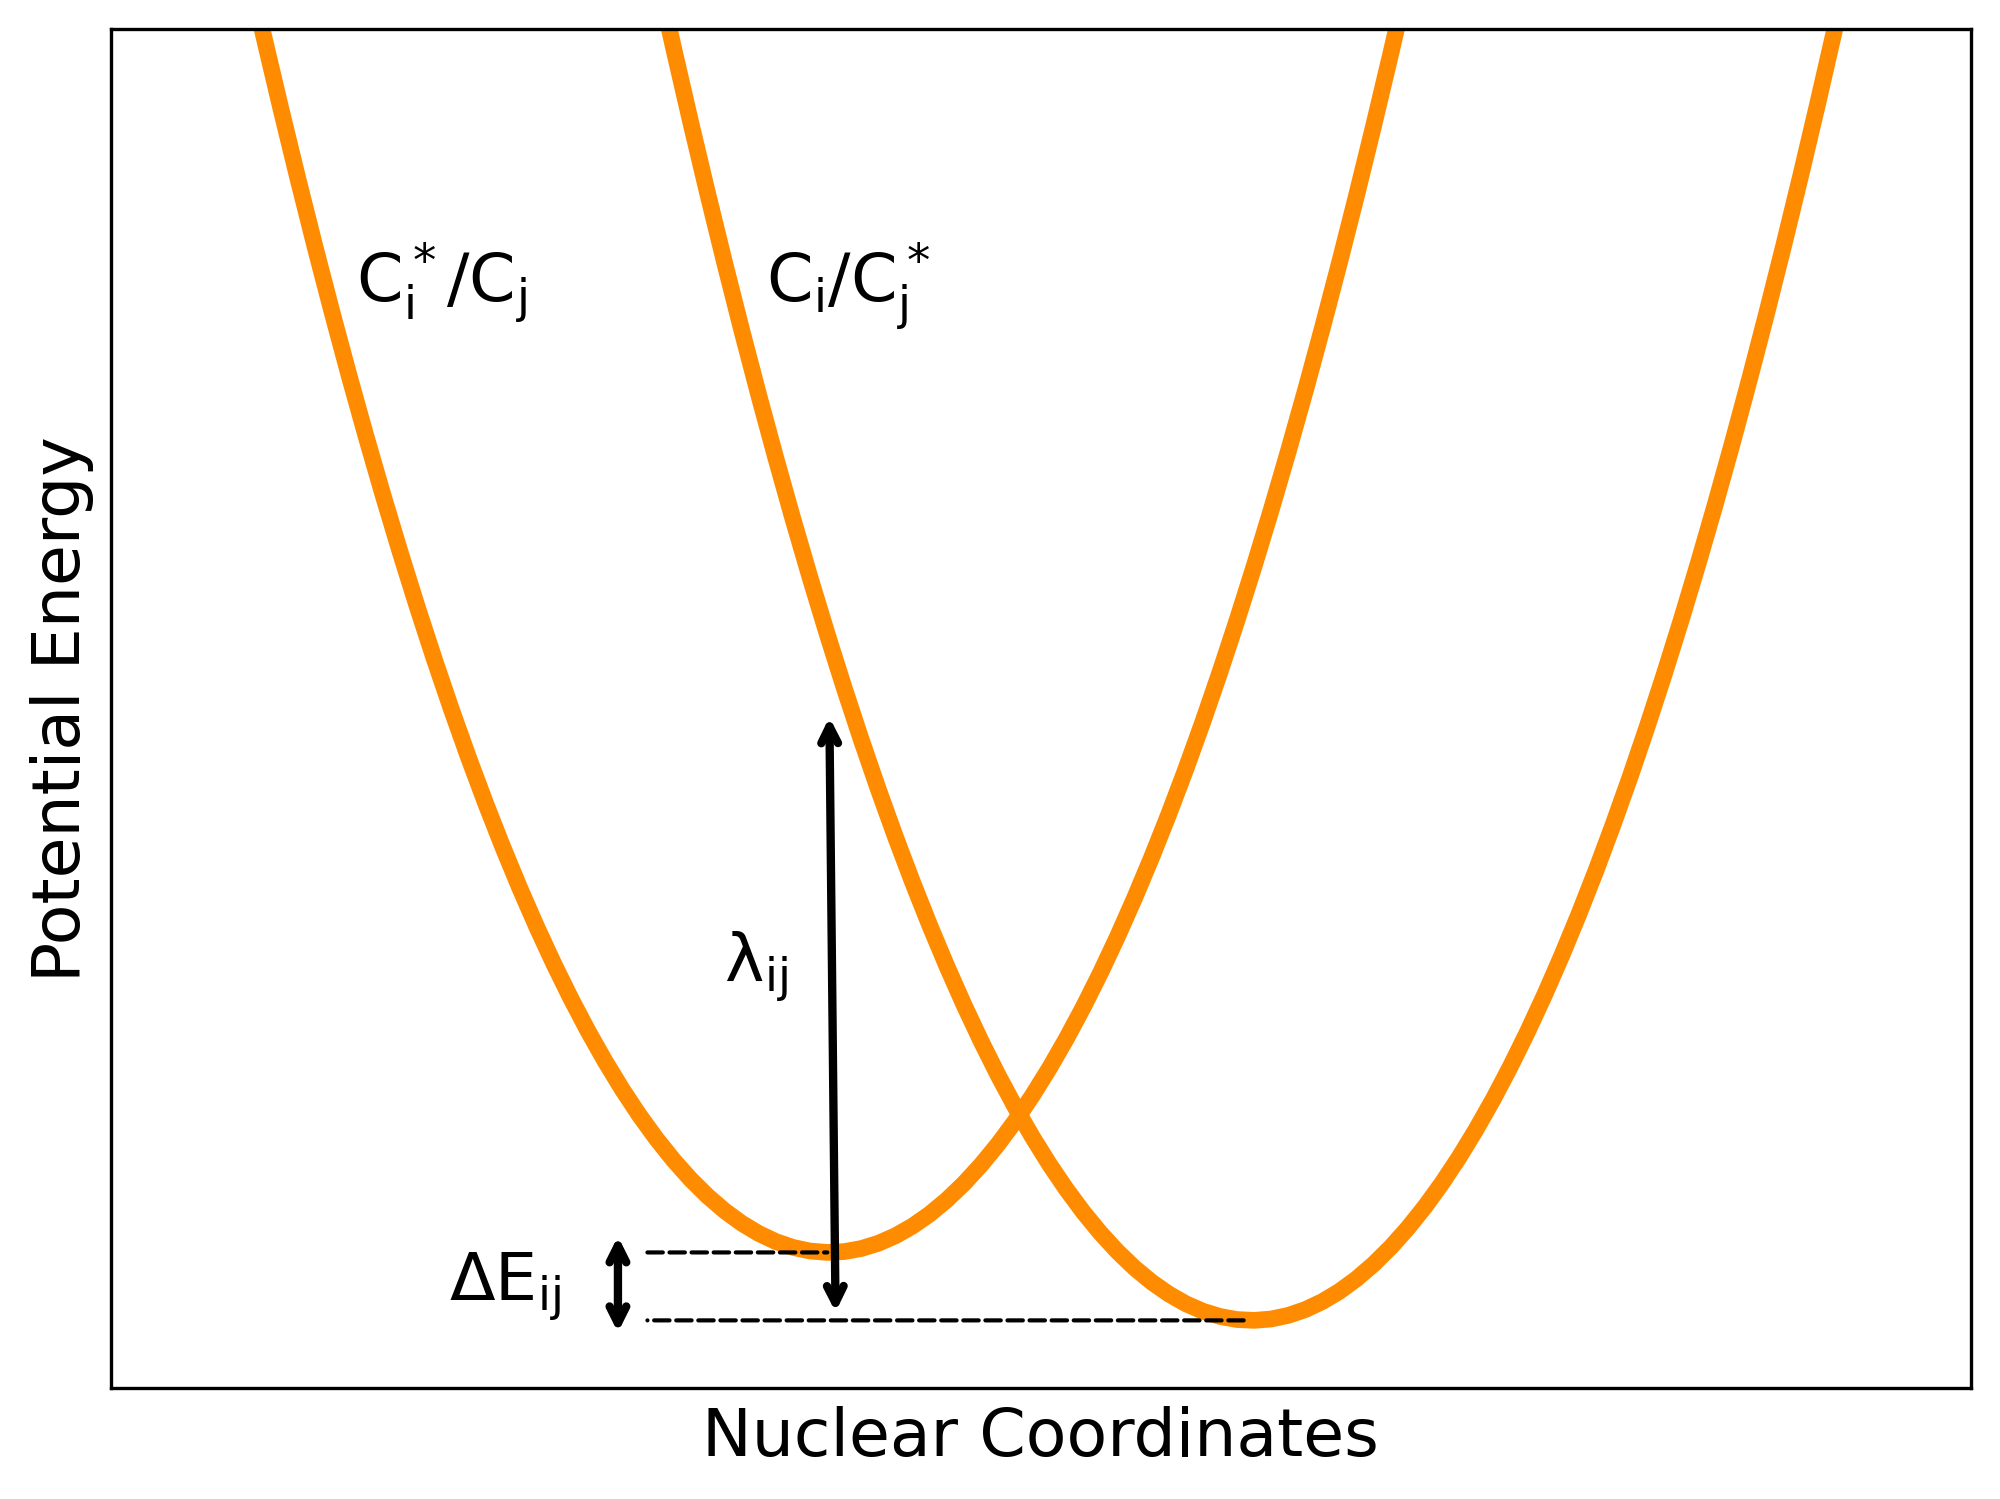
\includegraphics[width=0.7\linewidth]{figures/marcus-plot.png} 
    \caption{Two intersecting dimer potential energy surfaces annotated with $\lambda_{ij}$, the
    reorganization energy, $\Delta E_{ij}$, the free energy difference bewtween dimers. $C_{i}^*/C_{j}$ 
    and $C_{i}/C_{j}^*$ the dimer with charge on chromophore $i$ and on chromophore $j$ respectively}
  \label{marcus-plot}
\end{figure}

Within this framework, the rate at which a charge will hop from chromophore $i$ to chromophore $j$, $k_{ij}$,
is given by the following equation:
\begin{align}
    k_{ij}  =  |T_{ij}|^2\ \frac{2\pi}{\hbar \sqrt{4 \pi \lambda_{ij} k_{B} T}}\ \exp{\Bigg[ \frac{(\Delta
    E_{ij} - \lambda_{ij})^2}{ 4 \pi \lambda_{ij} k_{B} T} \Bigg] }
    \label{marcus}
\end{align}
with Boltzmann's consant, $k_{B}$, and Planck's constant, $\hbar$. The parameters $T_{ij}$, $\lambda_{ij}$,
$\Delta E_{ij}$, $T$ represent the electronic overlap, the reorganization energy, the free energy difference
between chromophores, and
temperature. These are discussed individually in the results section, wherein we test the sensitivity of
the KMC results to the choice or computaion of these parameters individually.
The accuracy of the Marcus rate is thus dependent on the accuracy with which the inputs can be estimated. In
our work, $\lambda_{ij}$ and $T$ are set as constants. In
the following section we outline our quantum chemical treatment of both $T_{ij}$ and $\Delta E_{ij}$ for all
potential hops throughout the morphology.

Computationally, simulating a charge hopping around a morphology requires identification of
individual chromophores and calculating the rate at which a charge will hop to neighboring
chromophores. 
Each local molecular environment requires its own justification for where chromophores in the morphology 
can be considered to harbor a localized free charge.

In disorderd organic systems, unlike in metals or single crystal organic materials, 
electronic states are localized to the frontier molecular orbitals of tightly
bound packets of atoms within the morphology. 
The spacial extent of chromophores is therefore dependent on the local environment of individual chromophores
and correspond roughly to the boundary between packets of strongly interacting molecular regions.

For ITIC, the candidate location of chromophores naturally arises from its composition of distinct
macromolecules.
The charges are taken to be localized on inividual molecules of ITIC. The frontier molecular orbitals have 
negligible electron density along the side chains. Therefore, the simplest model for chromophores then is
taken to be the backbone of individual molecules. Significant computational resources 
can be conserved by leaving the side chain atoms out of the of the QCCs. 
To test this on ITIC, we delineate the backbone and the whole molecule and compare carrier mobility in \autoref{itic}.
 
In the case of conducting polymers like P3HT this boundary is affected by the how the chains are twisted
or bent. A material that spans the gambit of disorder and crystallinity can be difficult to model, because
charge transport can occur in a hopping way, as described here, and also occur in an adiabatic metal-like transport. 
Therefore, while experimental studies have suggested that charges localize along roughly 7 monomer chains
in P3HT, our application of our model to three morphologies of P3HT with vastly different structure mean 
that this may not be broadly applicable. To disambiguate the results in this thesis we chose to take the
simplest model. Individual monomers in the system to be chromophores. The single monomer chromophore model has been shown to
produce good results \cite{jones2017}.
%%\ej{In this paragraph you should be talking about what charge delocalization is, show some examples of big and small chromophores from the literature, then state the facts about P3HT. THEN we can talk about how choosing chromophores is also a modeling choice: We could do 7-mers of P3HT as a chromophore, but then we're in the awkward situation of modeling hops down a chain where either (a) we have to think about a chromophore losing one monomer at the tail and adding a monomer at the head, or (b) we chop up polymers into 7-mer-chromophores which may not evenly divide into the chain lengths we're using. PLUS charge delocalization depends on the structure of the chain (what if the chain is super twisted? or bent??), so we chose to model P3HT charge hopping along individual monomers (a) because it was a simpler implementation than the above alternatives and seems reasonably justified, (b) as a test to see if it works at all. It does OK!}

Deciding where a chromophore should be expected is one step in the workflow that requires nuanced
scientific justifications. However, after that decision has been made, the significant procedural hurdle of 
computationally ascribing the atoms to their respective chromophores remains. 
Every atom in the MD morphology has a unique index. All of the methods that follow hinge on assigning the prescribed atom indices to their respective chromophore. 
In this work, we manually index these chromophores. A tutorial for using VMDs graphical user interface to
visually select chromophores is maintained for \texttt{MorphCT}.
We also maintain workflows for automating the identification of chromophore positions using smarts
matching.

With the morphology chopped into chromophores and stored in memory, the energetics between
neighboring chromophores can be estimated with quantum chemical methods.

\subsection{Quantum Chemical Methods}
\label{qccmethods}

Calculating the rate at which a charge hops from one chromophore to the next
using Marcus theory requires an understanding of the energy changes associated with the hop, 
which requires a calculation of chromophore's electronic orbital structure.
Quantum chemistry allows for the estimation of the energy levels of electrons (holes) whose molecular orbitals 
are implied by the chromophore's current atomic configuration. 
Quantum chemical calculations comprise a set of methods, including \textit{ab initio} calculations implemented 
in Density Functional Theory packages that work from first principles, 
and semi-empirical methods that use experimental data to make modeling approximations \cite{Cui2014a}.

We assume that the electrons occupying the frontier molecular orbitals are the sole participants in the
hopping that is going on between chromophores. That is, if an electron hops from $i$ to $j$, it will hop
into the lowest unoccupied molecular orbital (LUMO) of $j$, and out of the
highest occupied molecular orbital (HOMO) of $i$.
The driving force for a one electron charge transfer reaction, 
with a rate described by \autoref{marcus}, is the difference between the energy that our electron 
currently posseses 
on chromophore $i$, and the energy that it could enjoy over on chromophore $j$. 
This is writtin as follows:
\begin{align}
    \Delta E_{ij} = E_{homo, i} - E_{homo, j}.
    \label{gibbs}
\end{align}
Quantum chemically, the values $E_{homo, i}$ and $E_{homo, j}$ represent the eigenvalues of the the
time-independent Shrodinger equation corresponding to the HOMOs of chromophore $i$ and $j$ respectively. 
In our work, these values are approximated with the MINDO/3 method, a variation of the intermediate neglect of 
differential overlap (INDO) method. This method seeks recreate the \textit{ab initio} Hartree-Fock
results, where Hatree-Fock theory allows for an iteratively convergent numerical solution to the
Shrodinger equation \cite{Thiel2014}. 

The value $T_{ij}$ in \autoref{marcus} is a measure of the electronic orbital overlap between chromophores.
This values can be obtained using the
the dimer splitting methed~\cite{Huang2005b}. This method comares the HOMO energies of chromophores $i$ and
$j$ in isolation to the energies of the frontier molecular orbitals of a dimer
consisting of the two chromophores. 
This difference is written as ($E_{homo,dimer} - E_{homo-1,dimer}$) where $E_{homo,dimer}$ 
and $E_{homo-1,dimer}$ are the two highest energy occupied molecular orbitals of the dimer. MINDO/3 is used
again to approximate the eigenvalues of the frontier molecular orbitals, but this time of the dimer
Hamiltonian. 

The dimer method can be imagined as a dimer being pulled apart. At some distance
the two highest occupied energy levels of the dimer will 
be the HOMOs of their respective chromophores. \ej{I like it.}
If the chromophores are not interacting, 
then the two highest energy molecular orbitals of the dimer will be the HOMO of chromophore $i$ and the 
HOMO of chromophore $j$. If there is electronic overlap, a comparison bewteen the two highest occupied
molecular orbitals of the dimer and the HOMOs of the chromophores calculated in isolation can quantify the degree of
electronic overlap. Indeed, $T_{ij}$ is written as follows:
\begin{align}
    T_{ij} = \frac{1}{2}\sqrt{ (E_{homo,dimer} - E_{homo-1,dimer})^{2} - (\Delta E_{ij})^{2} }.
\end{align}
 
Solving shrodingers equation, with any level of accuracy,
across an entire molecular arrangment is a prodigious computational lift.
Other studies have implemented \textit{ab initio} DFT methods at this stage of predicting
mobility from molecular arrangement to good effect \cite{Deng2004}. These more rigerous methods are
untenable on the scale of the morphologies studied in this thesis. While INDO methods are less precise, 
the results of using this method have shown good agreement with experimental and \textit{ab initio}
DFT methods~\cite{Bredas2002}. 
Compuational quantum chemistry is a nascent and evolving field of its
own, with quickly increasing efficiencies and accuracies.
A particular 
choice of method comes down to how well we can organize a workflow and integrate the QQC portion of the
workflow modularly to facilitate upgrading the QCC as more effecient methods and/or software emerges.

In our implementation, a quantum chemical calculation must be performed for every chromophore and every chromophore pair. 
To understand the scale of this lift, the reader is reminded that
`n choose k' notation gives the number of ways to choose `k' objects from a set of 
`n' objects as follows 
\begin{align}
    {n \choose k} =  \frac{n!}{k!(n-k)!}.
\end{align}
Therefore, the upper bound of possible chomophore pairs (pairs setting $k=2$) is given by the 
$n \choose 2$ where $n$ is the total number of chromophores in the simulated volume. 
With this, the effort of exhaustively calculating all chromophore pairs scales as $\frac{n^{2} - n}{2}$, or using big Oh notation, $O(n^2)$.
This quadratic scaling of computational effort before performing kMC simulations can represent a bottlneck, so
we investigate and apply approaches for identifying and calculating only the chromophore pairs that are
spacially proximal.

In the following section we introduce our methods for determining
which chromophore pairs to consider using Voronoi analysis. 

\subsection{Voronoi Analysis}

To minimize the number of dimer calculations, we use Vornoi analysis to locate the spatially
nearest neighboring chromophores. This analysis is performed on the cartesian coordinates of
the geometric center of the chromophore. With that, a polyhedron cell is constructed around this geometric
center. The polyhedron cell consists of every point in space that is closer to that chromophore center than
any other chromophore center. Chromophores are considered neighbors if their voronoi cells abut one another.

For simplicity, we construct and visualize a Voronoi diagram of the xy components of the chromophore centers
of the crystalline P3HT system described in \autoref{md}. To carry out this analysis, \texttt{MorphCT} incorperates the
Voronoi class provided by \texttt{freud}; a python package for analysing and visualizing simulation data\cite{Ramasubramani2020}. 
This class is compatible with 2D or 3D simulation data. 

Shown in \autoref{fig:ln}, 15,000 thousand dots represent the chromophore's geometric centers projected
in the xy-plane. In this 2D analogue,
cell edges are drawn in a Euclidean way, with lines between polygons representing the set of points 
equidistant from that point and its geometrically closest neighbor across the line. 
In the 3D case, this analysis reduced the pairwise calculation from ${15000 \choose 2} = 112,492,500$
to $113,315$. 

Euclidean space searching algorithms of this sort are an effecient way to parse space. 
They are known to scale with $O(n\log{n})$ in the worst case and as low as $O(n)$ in the average case
\cite{Bentley1980}.


\begin{figure}
  \center
%\includegraphics[width=25cm]{figures/crystalline_voronoi.png}
  \includegraphics[width=0.99\linewidth]{figures/crystalline_voronoi_smaller.png} 
 % \includegraphics[width=\linewidth]{figures/crystalline_voronoi_smaller.png}
  \caption{A 2D Voronoi diagram that was drawn from the xy components of a crystalline P3HT morphology. Dots
    represent chromopore centers. Lines represent points that are equidistant to the chromophore centers.
    Polygons represent all points that are closer to the chromophore center contained within than any other
    chromophore center. RED SQUARE: \autoref{fig:dcut} shows the 15nm section of the sample zoomed in for
    detail.}
  \label{fig:2d}
\end{figure}
\begin{figure}
  \center
  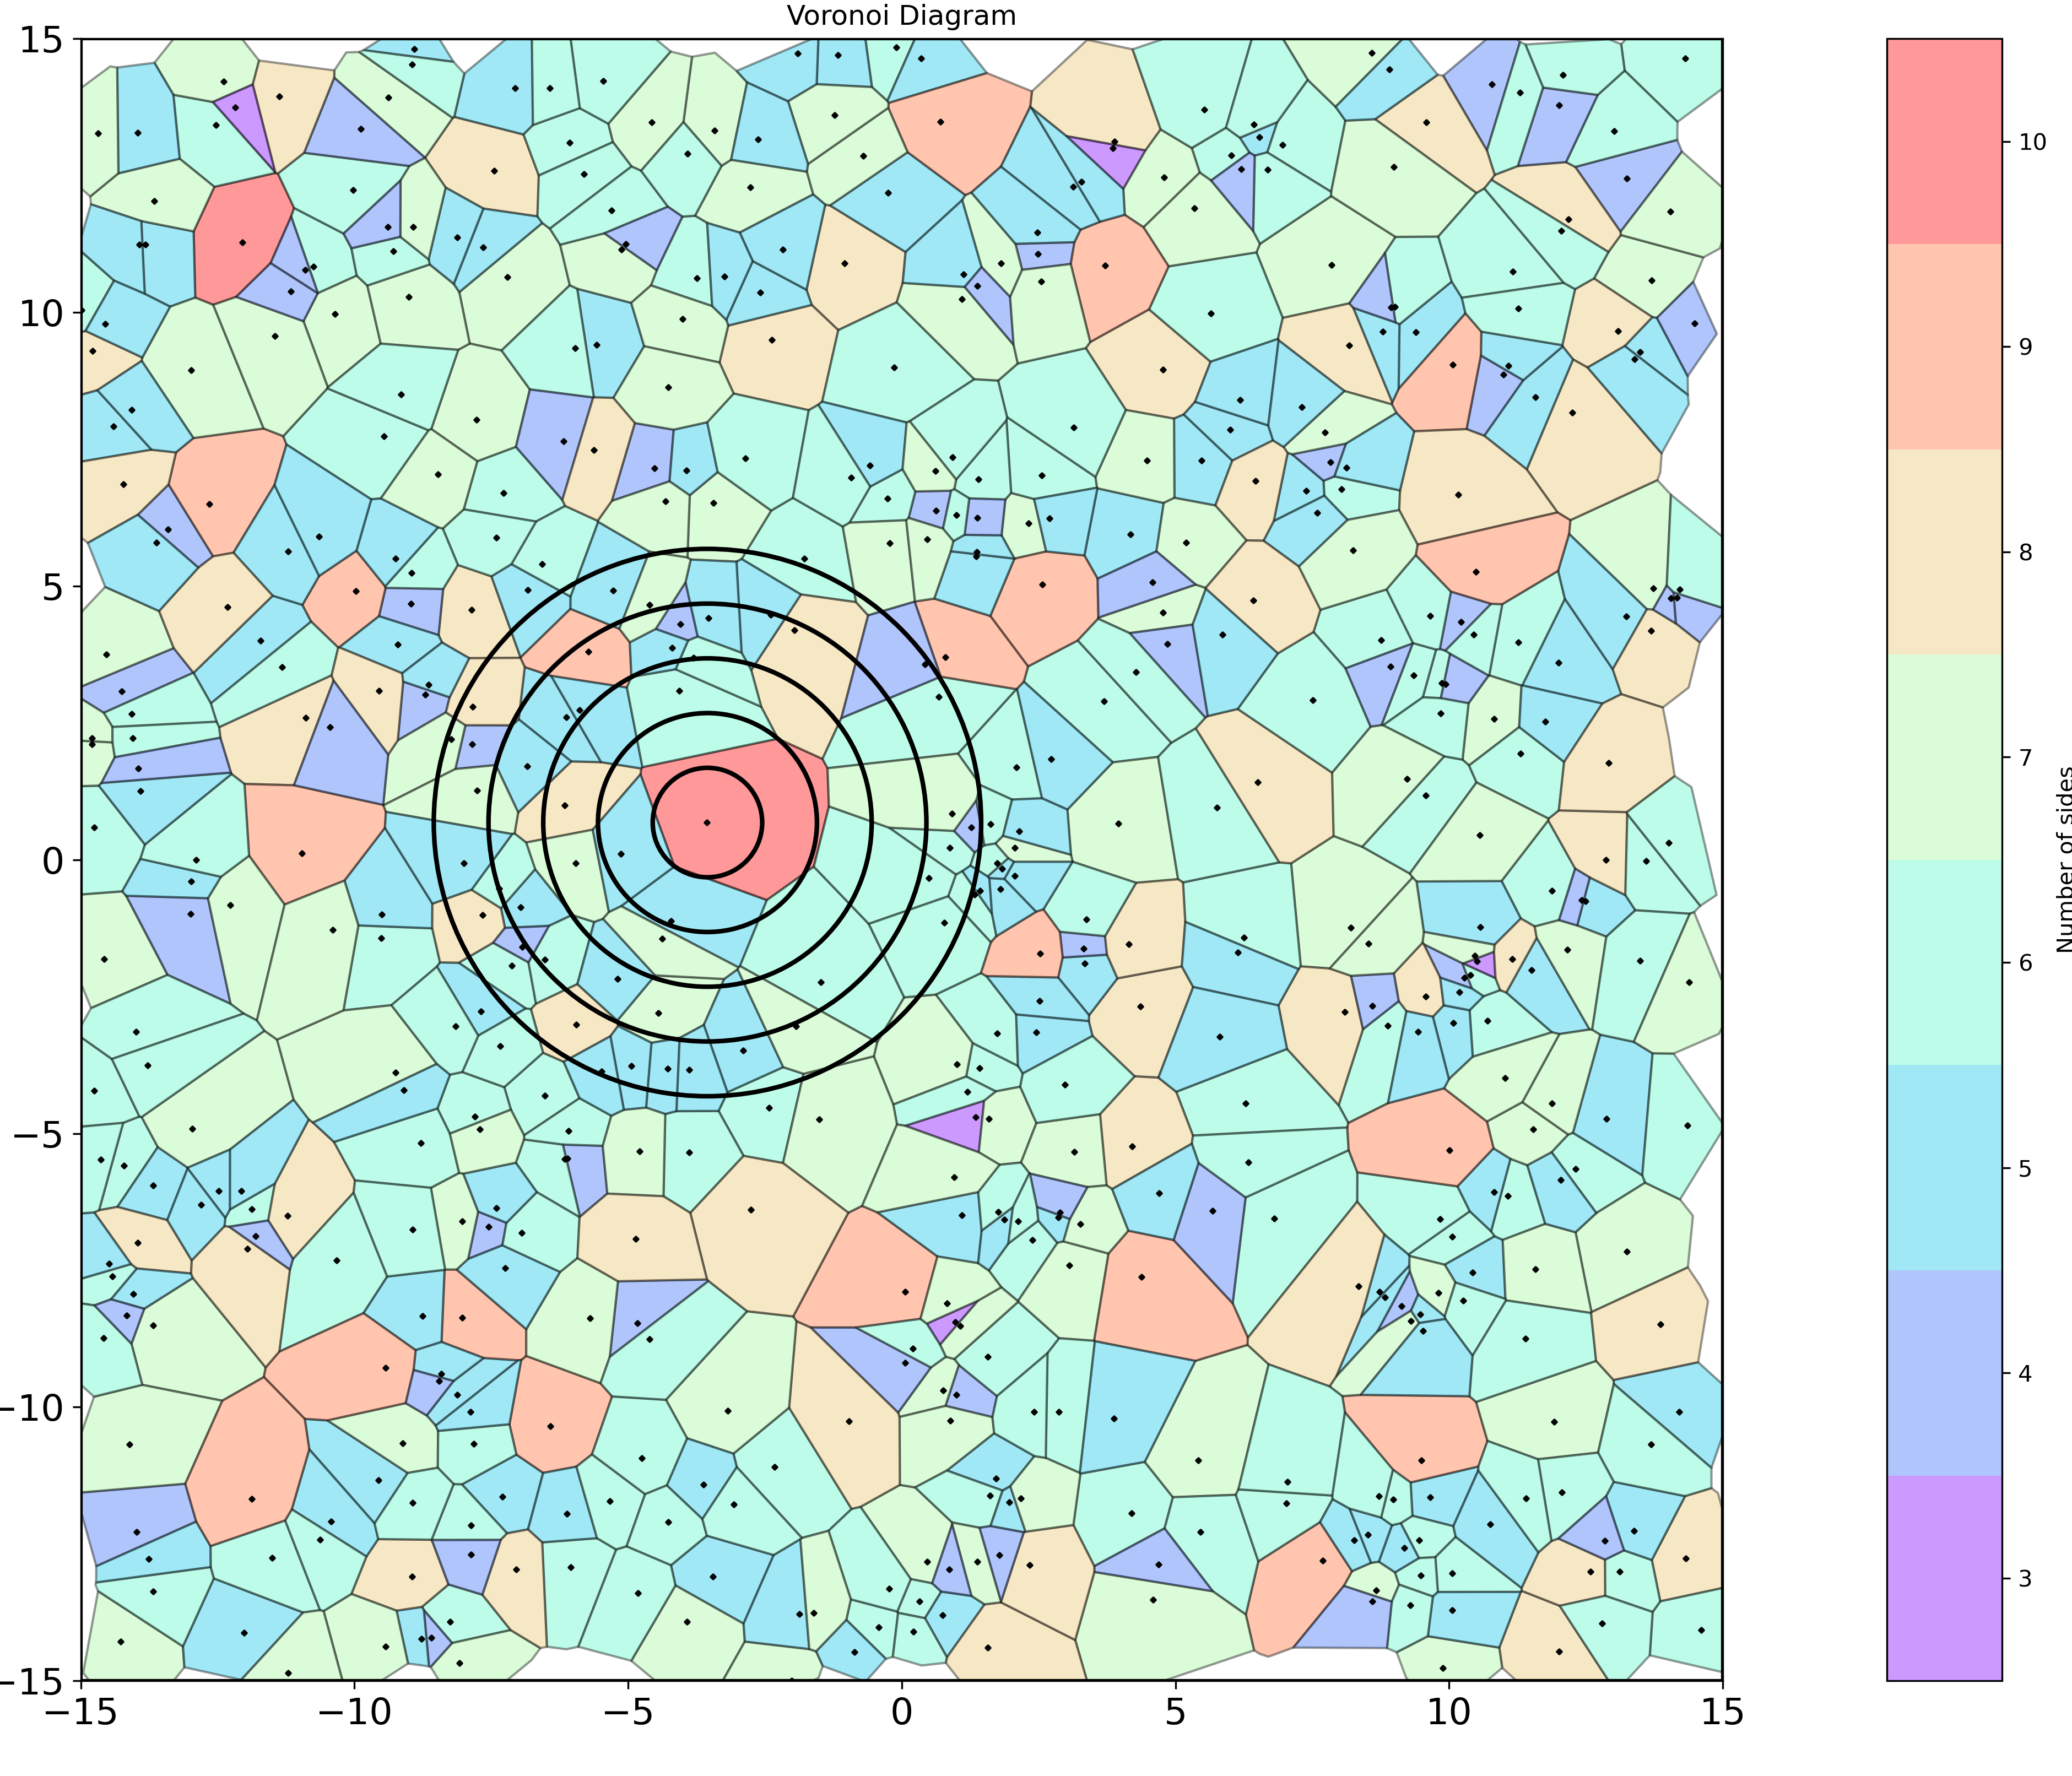
\includegraphics[width=\linewidth]{figures/crystalline_voronoi_d_cut_circles.png} 
    \caption{Zoomed section of \autoref{fig:2d} wherein we see a cartoonized version of a dcut radius cutoff
    used to suppliment Voronoi analysis. Circles represent the neighbor cutoff
    radius(dcut) beyond which we truncate chromophores from the neighborlist.
    Cells are colored by number of neighbors.}
  \label{fig:dcut}
\end{figure}

However, an artifact of constructing nieghborlists in this way is that some
neighbors are too far apart to interact electronically, but are nevertheless closer to each other than they
are to any other chromophores and are therefore counted as neighbors. 
Inspection of \autoref{fig:dcut} reveals how this phenomena can arise from this type of construction.
Because charges will not hop between these pairs, including them in the pair list will result in 
superfluous QCCs. 

In light of this, we introduce a parameter by which we further pare down the neighbor list. This parameter is
a naive cutoff distance, referred to as `dcut' in this thesis. We visualize various dcut values as black
circles in \autoref{fig:dcut}.
It is clear from this image that the choice of dcut is could drastically effect the
neighborlist.  
Note that the z-direction has been collapsed, and the distances do not necessarily correlate to the distance
between chromophores in the system.

A proper choice of dcut will depend on the material under investigation, 
as the size of the individual chromophores will vary. In 
\autoref{dcutresults}, we test the sensitiviy of our results to the value of dcut for the crystalline P3HT
data. From this testing, we consider if the juice is worth radial squeeze from a computational standpoint. 

\section{Kinetic Monte Carlo}
\label{KMC}

With the MD data generated, the data chopped into individual chromophores, 
the chromophores and chromophore pair energetics
quantified with QCC, and the Marcus hop rate calculated, 
a single charges movement through the morphology can be simulatied with the
application of a KMC algorthim.

Monte Carlo algorithms use pseudorandom numbers to solve computational problems. Our implementation can be
described as a first choice method KMC algorithm, where the kinetics involved is the rate of one electron
charge transfer reactions and the first choice is that of the fastest available hop for a given charge.

Using \texttt{MorphCT}, a charge is implanted as quasi-particle into a random chromophore within 
the morphology. In this model, we assume that the only events that can take place in the system are hops
between chromophores. With this, the rate of all possible events in the system are known and are given by
\autoref{marcus}. 

With the charge implanted, the hop rate, $k_{ij}$, from the occupied chromophore to any
given neighboring chromophore is taken to be
inversely proportional to the amount of time, $\tau$, that the system will have to wait before that hop will
take place. The $\tau$ of all available hops forms a queue of hops from shortest wait time, fastest hop, to
longest wait time, slowest hop. From this queue, the shortest wait time (first choice) can be selected
and the system can be moved forward in time by $\tau$.

However, hopping processes at the angstrom level do not proceed deterministically. 
Our implementation, and others like it [NEED REFS?], have
successfully captured the stochasticiity of these systems via a shuffling our hopping queue.
The shuffled wait time for every potential hop from occupied chromophore $i$ onto a
neighboring chromophore $j$ looks as follows:

\begin{align}
    \tau = \frac{1}{k_{ij}} \cdot \ln{\frac{1}{x}} 
    \label{waittime}
\end{align}
where x is a random number between 0 and 1 and $\log{(1/x)}$ is a scaling factor. To illucidate this
graphically, $\ln{(1/x)}$ is plotted in figure \ref{fig:ln} from 0 to 1. From this we can see that with
a large enough sampling, significant reshuffling of the queue will take place, allowing for a rare hop to jump
the queue.

\begin{figure}
  \center
  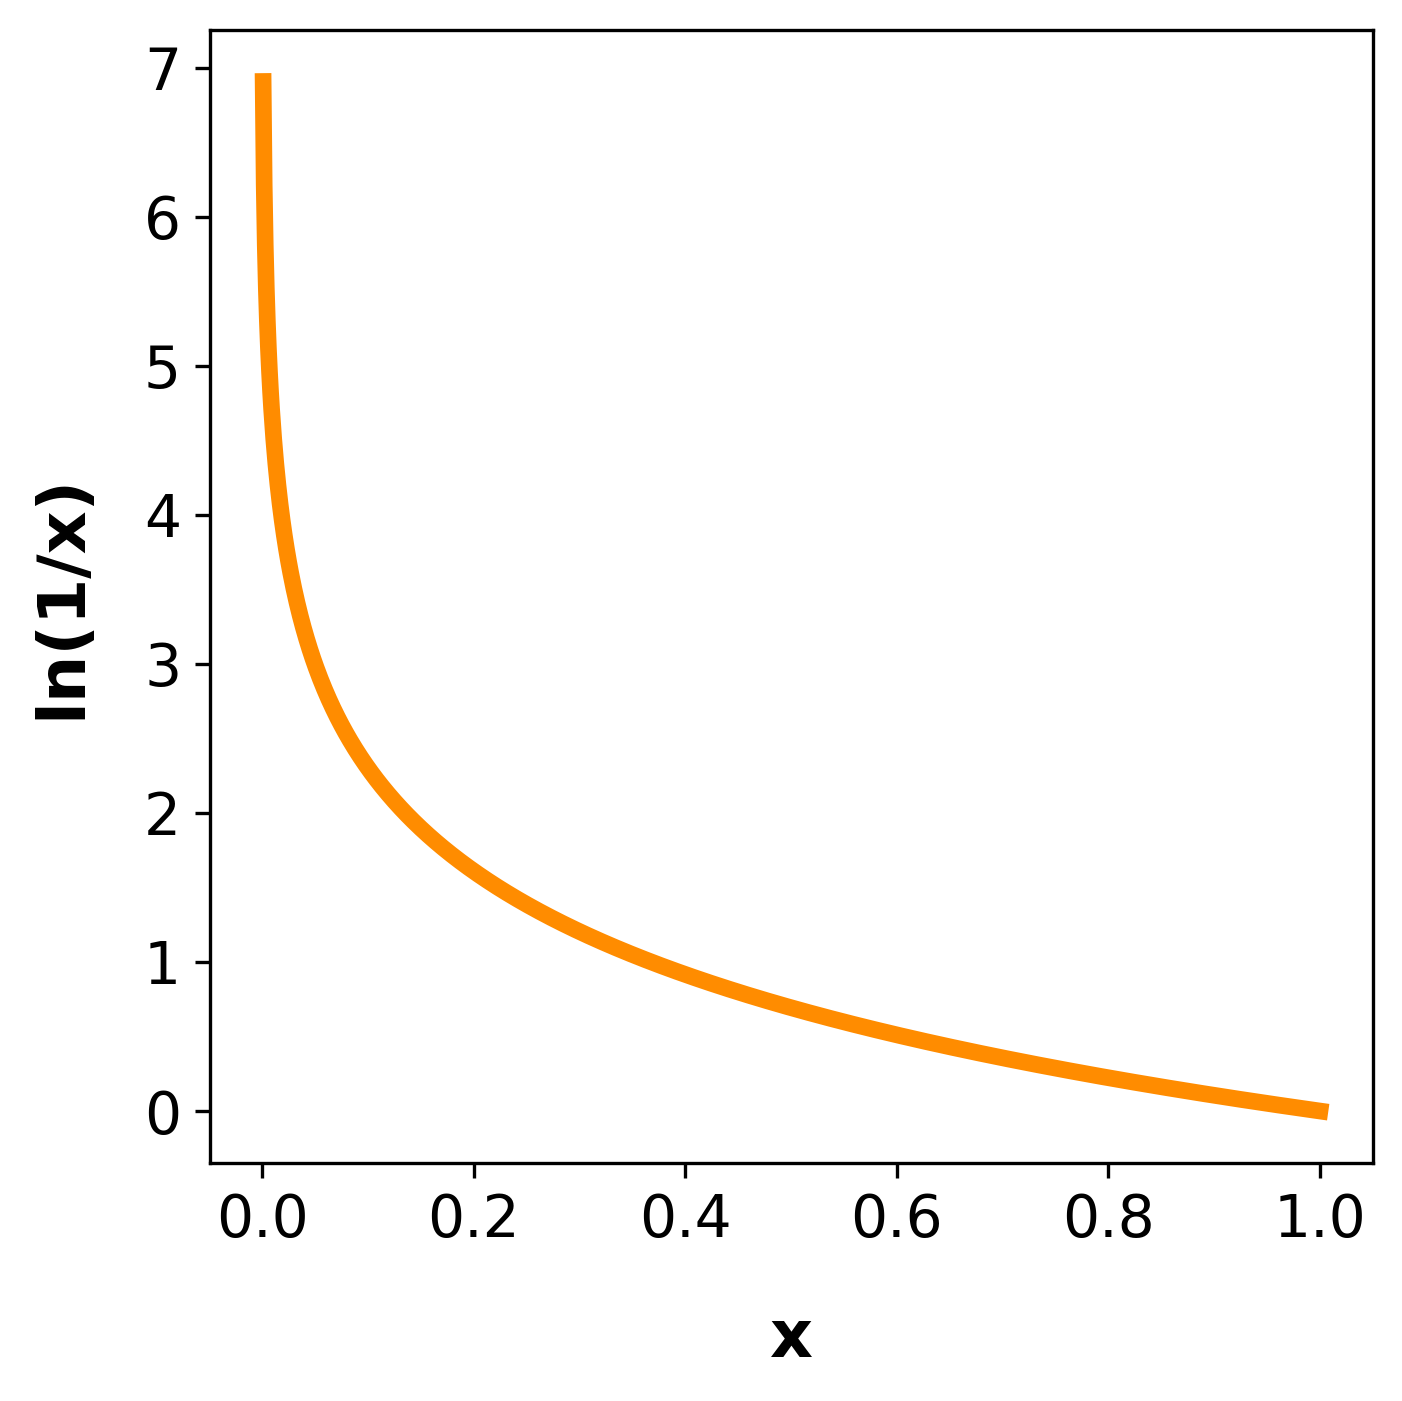
\includegraphics[width=0.8\linewidth]{figures/naturallog.png}
  \caption{Graphical insight into the reshuffling of the wait time queue. Here the x-axis represents the 
    interval from which numbers are drawn randomly such that the wait times in the queue can be scaled 
    by ln(1/x).}
  \label{fig:ln}
\end{figure}

From the rationally shuffled queue, the shortest waittime is chosen and the charge is moved to
its new chromophore host. The system is then considered to have moved forward in time by $\tau$. This proceeds
until the charge carrier stalls out or hops past a prespecified lifetime. How we aggregate data from 1000's of
single KMC simulations to obtatin macroscopic charge mobility is the subject of the following section.



\subsection{KMC analysis}

\label{kmcanalysis}

\texttt{MorphCT} allows for the creation of a system object that holds all the information necesarry to carry out the
KMC simulations outlined above. Running the simulation requires the choice of three system parameters: the
KMC temperature, the number of indivual KMC simulations to perform, and the charge carrier lifetimes. 

The choice of carrier lifetimes effectively serve as checkpoints at which the displacement of charge carriers is recorded. For
each specified lifetime, the prescribed number of individual KMC simulations is run as in \autoref{KMC}. When a
given charge carrier hops past the specified lifetime, that is, the addition of the current iterations $\tau$ advances
the simulation beyond the specified lifetime, 
its displacement from its starting location is stored in the carrier object. After repeating this over a
statistically significant number of carriers, the carrier data can be aggregated and the mean squared
displacement (MSD) for particles over that amount of time can be calculated. MSD over a given time period is 
the standard deviation in position for a free charge walking randomly through this electronic environment. 

It is known that the MSD of a diffusive particle increases linearly as time goes to infinity. 
The slope of the MSD, $D$, as time
goes to inifinity can be estimated as a linear fit between the MSD of charge carriers at the specified lifetimes.

There is no objective best practice for determing the slope of the MSD as
time goes to inifinty from simulation data of this kind \cite{Maginn2018}. With that, we seek primarily to
simplifiy the MSD analysis as much as possible. Doing so will make for more accurately reported results and
easier apples to apples comparisons with future results. 

Finally, the results of the MSD analysis are then used to determine the zero-field mobility using the following Einstein-Smoluchowski relation:
\begin{align}
    \label{einstein}
    \mu_{0} = \frac{eD}{6k_{B}T},
\end{align}
where $e$ is the elemental charge of a charge carrier, $D$ is the diffusion coefficient, $k_{B}$ is Planck's
constant and $T$ is temperature. 

The conductivity of a material given by 
\begin{align}
    \label{conductivity}
    \sigma = n \cdot e \cdot \mu,
\end{align}
where $n$ is the number of charge carriers, $e$ is the charge of an electron and $\mu$ is empirically
defined as drift velocity, $v$, over the electric field, $E$ as follows \cite{Kokil2012}:
\begin{align}
    \label{m}
    \mu = \frac{v}{E}
\end{align}
With that, our KMC simulation most closely models a measure of conductivity in a bulk material in a controlled
environment. That is, conditions wherein \autoref{conductivity} is measured with negligible $n$ and $E$.
This is the case for time-of-flight experiment carried out on very thin films under low charge density
conditions \cite{Chen2000a}.

A benifit to Monte Carlo analysis of this type is that charge carriers can be simultaneously. It is considered
to be ``embarrasingly parrel'' in that the subprocesses (charge carriers) require no communication.

\section{Software Development}

\label{software-methods}
% this section should be about about HOW we develop software? Using version control, pull requests, 
%jupyter notebooks, continuous integration, tests, and validation? This can given in the context of true
%After all, how we do things is a method.
%action: made a NEW section for this and morpchct in general

We manage development of the \texttt{Planckton} and \texttt{MorphCT} software packages using public repositories hosted at
github.com\cite{cmelab} for the excecution of these methods.
As with any open-source software project, these repositories serve as a
central hub for developers to collaberate and integrate code into the code base. Repositories are
version controlled with a snapshot of the code base saved at each iteration. This allows researchers to 
reproduce each others work with the exact version used to carry out the analysis. It also provides a
documented and controlled way to merge together divergent code through pull requests. Unit testing and
continuous integrationg techniues provide passive protection against bugs in the software that might emerge
from active development on the code base. 

Modular, python based code allows for the curation and publication of Jupyter notebooks workflows and
tutorials for performing reproducable analysis. Jupyter notebooks are a document format for publising code
that is excecutable and interactive \cite{Kluyver2016}. 

 

\begin{table}[]
    \caption{Packages} % title of Table
\centering % used for centering table
\begin{tabular}{|l|p{0.8\linewidth}|} % centered columns (4 columns)
\hline\hline %inserts double horizontal lines
Package/tool & Description \\ [0.5ex] % inserts table
%heading
\hline % inserts single horizontal line
    \texttt{foyer} & python package for applying atom-typing rules  \cite{Klein2018a}\\ [1ex] % inserting body of the table
\texttt{freud} & python package for analyzing particle simulations  \cite{Ramasubramani2020}\\ [1ex] %
\texttt{HOOMD-Blue} & general purpuse toolkit for performing simulations.   \cite{Anderson2020a}\\ [1ex] %
    \texttt{mBuild} & python based molecule builder \cite{Klein2018a}\\ [1ex] % [1ex] adds vertical space
\texttt{MorphCT} & python package for simulating and analyzing charge transport from 
    snapshots of MD simulations \cite{jones2017}\cite{cmelab}\\[1ex] 
OVITO basic & tool for visualiztion simulation data \cite{Stukowski2010a}\\[1ex] 
\texttt{packmol} & python package for creating initial configurations of simulations \cite{Martinez2009}\\[1ex] 
\texttt{Planckton} & python based convenience package for running \texttt{HOOMD-Blue}
    simulations of OPVs \cite{cmelab}\\[1ex]
    \texttt{Planckton-flow} & python based package that supports the use of \texttt{Planckton} on
    high performance clusters\cite{cmelab}\\[1ex]
\texttt{pySCF} & open-source collection of electronic structure modules \cite{Sun2018a}\\[1ex]
\texttt{signac} & python based framework for managing large heterogenous data spaces \cite{Adorf2016}\\[1ex]
VMD & a molecular visualization program for displaying, analyzing, and animating large biomolecular
    systems \cite{Humphrey1996}\\


\hline %inserts single line
\end{tabular}
\label{packages} % is used to refer this table in the text
\end{table}

Having had no prior experience with these materials and/or materials simulation prior to joining the CMElab,
I was able to take an investigation of ITIC from molecular
structure to a charge mobility; a macroscopic property. We hope that the combination of these two packages
can make in silico screening of OPV materials realistically attainable by any aspiring researcher.

All the tools used to implement, analyze, and
visualize this work are freely available. 
The packages and tools are enumerated in \autoref{packages}. We now describe \texttt{Planckton} and 
\texttt{MorphCT} in more detail.

\subsection{MD Software}

\label{planckton}

\texttt{Planckton} is a convenience package that integrates, \texttt{Mbuild}, \texttt{foyer},
\texttt{HOOMD-Blue} for performing MD simulations of self-assembly in OPVs.  \texttt{Planckton}
provides clearly documented template scripts for inititializing and running MD simulations. 
 
\texttt{Planckton} uses \texttt{foyer} to interpret the forcefields used to generate the MD data. The MD
simulations performed for this thesis employ the Generalized Amber Force Field (GAFF)\cite{Wang2004}.
The Amber forcefield was designed for use in modeling protein and
nucleic acid systems. Serendipitously, the generalized Amber forcefield has parameters for organic molecules
comprised of H,C,N,O, and P and can produces accurate simulations of organic molecules for use in OPVs. 
Also provided are files that define the atomic structure of many of
the most commonly studied OPVs for OSC research in a format that are compatible with GAFF forcefields.

\texttt{Planckton} is built using \texttt{HOOMD-Blue} simulation toolkit \cite{Anderson2020a}.
The native file format of \texttt{HOOMD-Blue} is the GSD file. GSD files store simulation data in a binary file. 
As MD simulations proceed, the GSD files are populated with the microstate of the system at regular intervals.
\texttt{MorphCT} is developed to operate on particular microstates stored in GSD files.

Containers are virtual machines that contain all the dependencies, configurations, code and data 
necessary to reproduce results \cite{Cito2016a}. 
\texttt{Planckton-flow} is a dataspace manager that uses
singularity \cite{singularity2017} and \texttt{docker} \cite{Merkel:2014:DLL:2600239.2600241} 
to `contanerize' \texttt{Planckton} \cite{cmelab}. \texttt{Docker} images are binary files that contain the
entire software stack necessary to execute some code. This allows researchers to minimize dependency issues
and increase reproducibility. However, \texttt{docker} has no native support for the use of GPUs and is not
compatible with the more draconian permissions often present on HPCs. With that, \texttt{Planckton-flow} uses 
\texttt{singularity}, a software designed to overcome these shortcomings,
to pull a \texttt{docker} image of \texttt{Planckton} to a container on the server. 

\texttt{Planckton-flow} allows for a container of \texttt{Planckton} to be taken 
off the shelf an pulled to performance computing cluster without having to build the software stack or write the
simulation scripts from scratch. Screening OPV materials across many thermodynamic parameters can results in
cumbersome data sets. \texttt{Planckton-flow} automates the management of large these large multidimensional
data sets with \texttt{signac}.

\subsection{KMC Software}
\label{morphct}

\texttt{MorphCT} is a package for running KMC simulations of charge transport in organics systems.
\texttt{MorphCT} operates on data containing the cartesian coordinates and atom types of particles in a
system. We operate \texttt{MorphCT} on equillbrium microstates obtained from MD simulations. However,
\texttt{MorphCT} is indifferent to how the morphological data was obtained and does not measure physical
accuracy of that data. 

In the delevopment of \texttt{MorphCT-flow} for analogous reasons to those outlined for \texttt{Planckton}, we
found that ORCA, the software used to perform QCC in \texttt{MorphCT} inhibited containerization because it
requires a licsensing agreement. ORCA was replaced with the fully open source pySCF. 
The software we have chosen to perform our QQC is
provided by \texttt{pySCF} (Python-based Simulations of Chemistry Framework) \cite{Sun2018a}. This framework
was chosen in the interest of reproducability and extensibility.
\texttt{pySCF} is implemented almost entirly in the Python 
language, which is becoming increasingly ubiquitous in the scientific computing community. The modularity of
\texttt{pySCF} allowed for the entire QQC code to be implememted in five lines of code. These lines of code in 
asked asks \texttt{pySCF} to approximate the frontier energy levels given the chromophore's molecular arrangement.  

\texttt{MorphCT} utilizes the python multiprocessing module to divide the prescribed number of charge carriers to be
simulated accross all available cores.

These workflows, maintained as jupyter notebook tutorials, 
are meant to lower the cognitive load of taking on a research project in this vein. 


%%% Local Variables: 
%%% mode: latex
%%% TeX-master: "BSUmain"
%%% End: 
